\chapter{Background and related work}

\section{Software-defined network}
\label{Software-defined network}
Software defined network (SDN) is a dynamic, manageable and cost-effective next-generation network structure. It is designed to deal with large scale, complex, dynamic data center network existing today. There are a lot of new concepts behind SDN. First of all, it is software programmable. One can configure, manage, and optimize network resources very quickly via automated SDN programs. For instance, companies are able to develop new applications that can further improve manageability. Secondly, it is very flexible. Abstracting control from forwarding lets administrators being able to adjust network-wide traffic flow to meet changing needs dynamically. Furthermore, a complete scope of the network is maintained by the central unit - controller, which is useful for application developing. It is also in charge of the flows inside the network. Finally, just like all other open source softwares, it is open standards-based and vendor-neutral. SDN simplifies network design because instructions are provided by SDN controllers instead of multiple, vendor-specific devices and protocols. To sum up, SDN provides greater visibility into network, reduces manual intervention, improves maintainability, and requires less hardware budget. Figure~\ref{SDN_struct} simply shows the architectural components of SDN, which are applications, network devices, Northbound and Southbound interface. In a SDN architecture, network devices are all\textit{switches} instead of \textit{switches and routers} in legacy network. In the following subsections, we will be looking at the structure of SDN.

\begin{figure}[H]
\begin{center} 
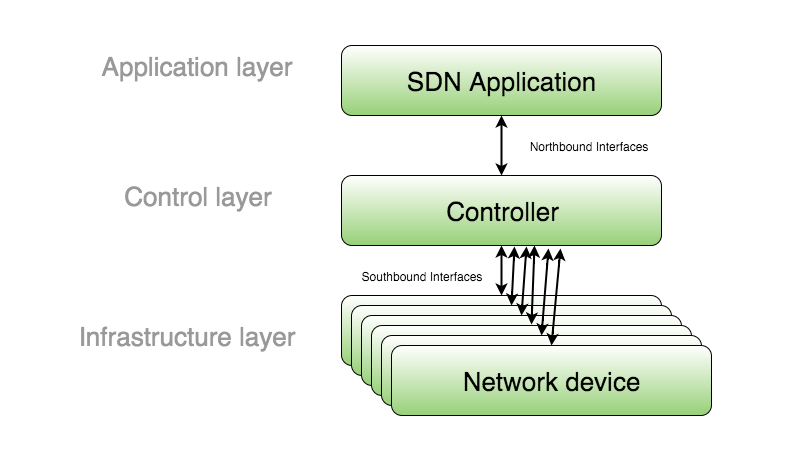
\includegraphics[width=0.85\textwidth]{figures/SDN_structure.png}
\end{center}
\caption{SDN architectural structure}
\label{SDN_struct}
\end{figure}

\subsection{SDN Application}
\label{SDN Application}
SDN applications are programs that communicate their requirements and desired behavior with the SDN controller via a northbound interface (NBI). An SDN Application consists of one SDN Application Logic and one or more NBI Drivers. They may consume an abstracted view of the network for their internal decision making purposes. Routing, Intrusion Detection System (IDS), firewall, network balancer, network monitor and modular composable service like FRESCO are all good examples of what one can build with SDN applications \cite{SPYFGT13}. These functionalities can be done at different layers of protocol stack.

\subsection{SDN Controller}
\label{SDN Controller}
The SDN controller is a centralized entity. It is responsible for managing the forwarding rules in every SDN switches and provides the abstract view of the network, including network topology and the state of network resources that SDN applications need. The interface for the communication between controller layer and infrastructure layer is called Southbound Interface (SBI). Some examples are OpFlex, SoftRouter, Puppet and OpenFlow \cite{LNRSW04}. OpenFlow is the first and most popular Southbound protocol for the time being. An SDN Controller consists of NBI Agents, the SDN Control Logic, and the SBI. NOX, POX, Floodlight, Ryu and Maestro are some open source controllers that are widely used \cite{GKPPCMS08,EZA11}.

\section{OpenFlow switch}
\label{OpenFlow switch}
OpenFlow is the first and most popular standard southbound interface. It enables network controllers to determine the path of packets by adding, modifying and removing matching rules in forwarding tables of the switches. It is able to realize more advanced network functionalities than routing protocols we use in legacy network. It allows switches from different vendors as long as the devices support OpenFlow. An \textit{OpenFlow Logical Switch} is a switch that support OpenFlow protocol. An OpenFlow switch consists of ports, flow tables and group table, Figure~\ref{OF_OV} is an overview of the whole OpenFlow switch structure. When a packet comes in from the \textit{ingress port}, it will go through flow tables, group table, and will be processed in corresponding to the matching flow entry. Aside from physical switches, there are also software implementations of virtual switch, such as \textit{Open vSwtich}. Typically, OpenFlow switches separate OpenFlow traffic and non-OpenFlow traffic with OpenFlow instances, they do not interfere with each other. \cite{HP_SPEC}

\begin{figure}[H]
\begin{center} 
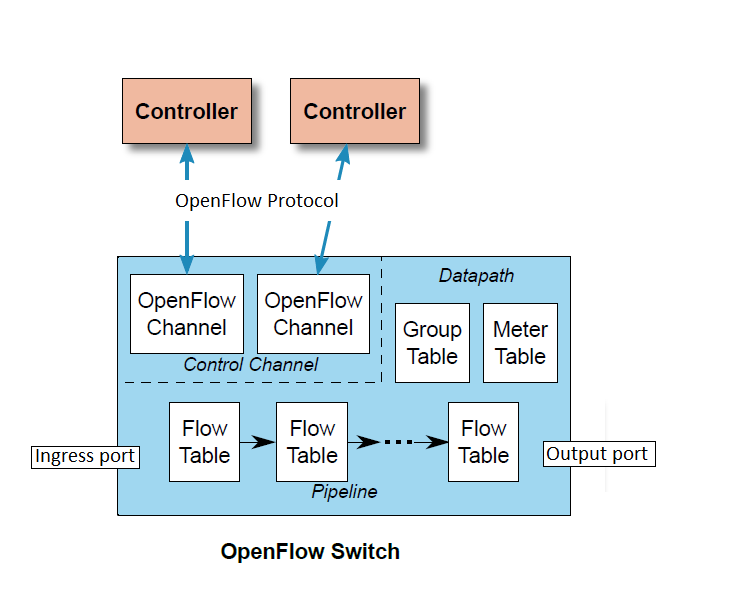
\includegraphics[width=1.1\textwidth]{figures/openflow_switch_overview.PNG}
\end{center}
\caption{OpenFlow switch structure overview}
\label{OF_OV}
\end{figure} 

\subsection{OpenFlow Channel and Control Channel}
\label{OpenFlow Channel and Control Channel}
The \textit{OpenFlow channel} is the interface for the controller to configure switch and receive packet from switch, and the \textit{Control Channel} on switches may support one or more OpenFlow channels, allowing more than one controllers to co-manage the switch. The connection may be initiated by either a switch or a controller. The OpenFlow channel is usually encrypted by TLS, but may be configured to run over plain TCP. The network used for OpenFlow channel can be either \textit{in-band} or \textit{out-of-band}. When using in-band network, it uses the network managed by the OpenFlow switch and is only logically separated from data plane, and the switch must set up the proper set of flow entries for the connection. If it uses out-of-band network, OpenFlow switches are connected to controller using separate dedicated network, and switches should make sure that the traffic of OpenFlow channel does not run through the OpenFlow processing pipeline. \cite{OF_SPEC}

\subsection{OpenFlow port}
\label{OpenFlow port}
OpenFlow switches are logically connected to one another by OpenFlow ports. Similarly to ports in traditional network, OpenFlow ports are the network interfaces for packets transmission. A switch sends and receives packets via ingress ports and output ports. There are two kinds of port. A \textit{physical ports}ports correspond to a hardware interface of switch, and a \textit{logical port} is higher abstraction ports that may map to various physical ports. When ports are added or removed, the content of flow tables remain unchanged. Packets forwarded to deleted or non-existent ports are just dropped, and if a same port number is reused after deletion, any remaining flow entries referencing to that particular number may be re-targeted to the new port, which possibly lead to undesirable result. Therefore, controller should clean up the reference of a port if a port is deleted \cite{OF_SPEC}. 

\subsection{OpenFlow table and entry}
\label{OpenFlow table and entry}
When packets arrive at a switch, it will go through the processing pipeline. In the pipeline, there are one or more \textit{flow tables}, and each packet is associated with an empty \textit{action set} at the beginning. Processing always starts with the first table in ingress processing. Each OpenFLow table contains multiple flow entries. Figure~\ref{FE_Col} is the columns of a flow entry. A flow entry is identified by its match fields and priority. Packets will be matched with \textit{match field}, which consists of ingress port, packet header and other optional pipeline fields. When a flow entry is matched, it will modify the action set according to its instruction. Some example of the actions are output to a specific port, drop and change TTL in the packet.

There is an entry with lowest priority that set all matching fields to wildcard, resulting in matching all value. When a packet does not matched by all other entries in all the flow tables, it is processed according to this entry. Normally it will be encapsulated and sent the the controller, the controller decides how it should be processed, and a new flow entry will be added according to the result.

If a flow entry does not specify next flow table, all actions in the action set are executed and the whole process inside the switch is complete. Egress processing happens after the output port is determined, its structure and mechanism is almost identical to ingress processing. It is an optional feature. If it is not enabled, the packet is then processed by output port and in most case forwarded out of the switch \cite{OF_SPEC}. 

Another type of OpenFlow table is called \textit{group table}. A flow entry may point to a group, providing additional method of forwarding. The columns of group entry is shown in Figure~\ref{GE_Col}. Each group entry is identified by a 32-bit unsigned integer as identifier. Group types specify how the many buckets should be executed in the group. Actions in an action bucket is applied as an actions set.

\begin{figure}[H]
\begin{center} 
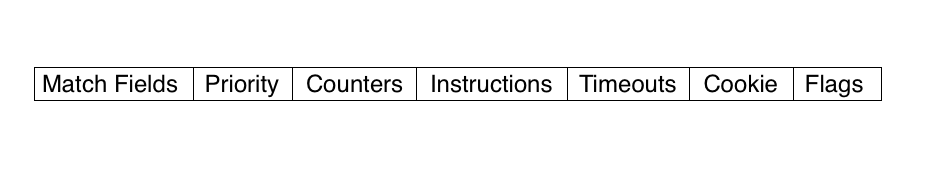
\includegraphics[width=1\textwidth]{figures/columns_of_flow_entry.png}
\end{center}
\caption{Columns of a flow entry}
\label{FE_Col}
\end{figure}

\begin{figure}[H]
\begin{center} 
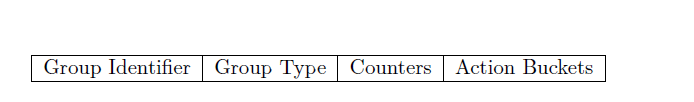
\includegraphics[width=1\textwidth]{figures/group_table.png}
\end{center}
\caption{Columns of a group entry}
\label{GE_Col}
\end{figure}

\section{Topology discovery services}
\label{Topology discovery services}
Topology managing in SDN is quite different from it is in regular network. To realize centralized control and high programmability, controllers need to maintain the visibility of the whole network. Therefore, topology discovery services play an important role in SDN. These services try to achieve auto adjustment when the topology alternate, which reduce the need of man effort significantly when it comes to network managing. The topology system include three parts: switch discovery, host tracking, and internal link. We will describe how these parts work individually in the following subsection.

\subsection{Switch discovery service}
\label{Switch discovery service}
When a switch try to initiate a connection with controller, the OpenFlow channel will be established just like we mentioned in~\ref{OpenFlow Channel and Control Channel}, the information of the switch will be sent to the controller and stored for future usage. 

\subsection{Host tracking service}
\label{Host tracking service}
Controller maintains Host Profiles to keep track of the location of a host. When a Packet-Miss happens like we stated in the second paragraph of~\ref{OpenFlow table and entry}, a Packet\_In message, along with the missed packet's information, will be sent to the controller. Then the controller will lookup the Host Profiles it maintains. If the Host Profile of the host cannot be found, controller assume a new host join the network and add this information. But if there is a conflict between the Host Profile and the Packet\_In message, the controller treat this as a host migration and update the location information of the Host Profile. Figure~\ref{HTS} is a illustration of host tracking service.

\begin{figure}[H]
\begin{center} 
\includegraphics[width=1\textwidth]{figures/Host_tracking.png}
\end{center}
\caption{Host tracking service.}
\label{HTS}
\end{figure}

\subsection{Link discovery service}
\label{Link discovery service}
When we refer to Link discovery, we mean the procedure of discovering the link between switches. Since there has not been a standard for the link discovery in OpenFlow controller, we will be using the term \textit{OpenFLow Discovery Protocol} (OFDP) when mentioning it. Currently, although there are be some minor difference in detail, all the main stream controllers support OFDP.

The OFDP leverages the Link Layer Discovery Protocol (LLDP) with subtle modification to perform topology discovery in an OpenFlow network. LLDP is originally implemented by Ethernet switch to exchange its identity and capabilities with a physically adjacent layer 2 peer, its EtherType field is 0x88cc. LLDP packets are sent regularly via each port of a switch \cite{LLDP_WS}. The information learned from received LLDP packets is stored by all the switches and the packets will not be forwarded after being sent across a single hop. Figure~\ref{LLDP_frame} shows the structure of LLDP Ethernet frame structure. Each LLDP Data Unit contains a sequence of type-length-value (TLV) like Figure~\ref{TLV}. As OFDP use a normal destination multi-cast MAC, OFDP advertisements would be forwarded by backbone switches. OFDP will not interfere with LLDP messages that the backbone networks may have implemented as it uses a different MAC address \cite{OFDP_GENI}. 

However, OFDP operates quite differently from LLDP. Just like we mentioned in the beginning of this section~\ref{Topology discovery services}, the topology information is kept by the controller instead of OpenFlow switch, and an OpenFlow switch will do nothing more than forward the LLDP packet. The simplified process is shown in Figure~\ref{OFDP}. All switches have a pre-installed rule in their flow table, sending any LLDP packet received from any port, except the controller port, back to controller via Packet\_In. Initially, controller creates an individual LLDP packet for each port on each switch via Packet\_Out message, each LLDP packets has their own Chassis ID. In the example figure, after receiving LLDP packet from controller, S1 sends it out on Port 1 and received by S2 on Port 3. As a result to the pre-installed forwarding rule, switch S2 forwards the received LLDP packet to the controller via a Packet\_In message. This Packet\_In message contains meta data such as the ID of the switch and the ingress port via which the packet was received. Thus, the controller can now infer that there exists a link between Port 1 of S1 and Port 3 of S2, and this information will be added to controller's topology database. After running this process through all ports on all the switches, controller is able to obtain all link between switches in the network. The entire discovery process is performed periodically with a typical default interval size of 5 seconds \cite{PPTI14}. 

\begin{figure}[H]
\begin{center} 
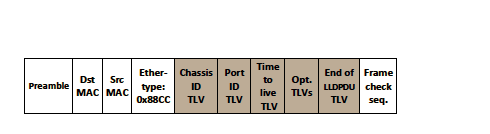
\includegraphics[width=1\textwidth]{figures/LLDP_packet_format.png}
\end{center}
\caption{LLDP packet frame structure. \cite{LLDP_WS}}
\label{LLDP_frame}
\end{figure}

\begin{figure}[H]
\begin{center} 
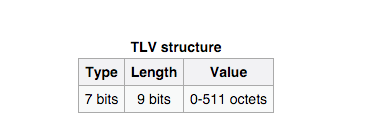
\includegraphics[width=1\textwidth]{figures/TLV_structure.png}
\end{center}
\caption{TLV structure. \cite{LLDP_WS}}
\label{TLV}
\end{figure}

\begin{figure}[H]
\begin{center} 
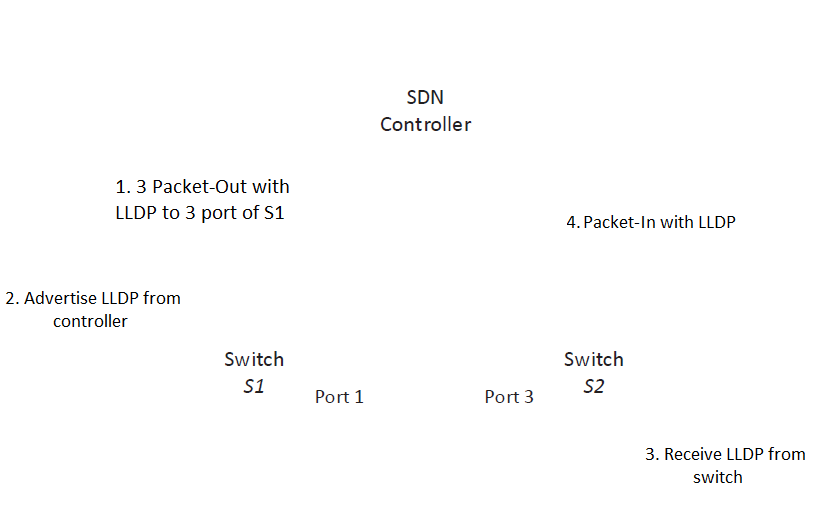
\includegraphics[width=1\textwidth]{figures/OFDP_procedure.png}
\end{center}
\caption{A illustration of OFDP procedure}
\label{OFDP}
\end{figure}

\section{SDN security}
As SDN brings fascinating development to network technology, its security has become a top concern. As a consequence of introducing a new structure, new protocols and new concepts, there will be more vectors that we should be concerned about in SDN. For instances, applications inside the controller might have flaws, control channel should be secured carefully, what a malicious host inside the network can achieve should be considered, and a lot more. And don't forget, beside those new elements, attacks may also happen in non-SDN-specific ways, such as system vulnerability exploit, administrative interface brute forcing etc. Figure~\ref{SND_threat_overview} is a whole picture of attacks we discuss and where they might possibly take place inside SDN, and Table~\ref{table:sdn_threats} contains further description of these threats with correspondent to their id number. In this chapter, we will talk about SDN security-related issues. We will focus on some of them and discuss about the attack scenarios, possible consequences and countermeasures. With all the wonderful features of SDN, we believe it is possible to come up with good solutions to deal with these security problems.

\begin{figure}[H]
\begin{center} 
\includegraphics[width=1\textwidth]{figures/SDN_threat_overview.png}
\end{center}
\caption{SDN threat overview.}
\label{SND_threat_overview}
\end{figure}

\begin{table}[H]
\centering
\caption{Detail of each attack.}
\begin{tabular}{|l|p{4cm}|p{3.2cm}|p{5cm}|}
\hline ID & Threat name	& Location & Consequences \\
\hline
\hline 1 & System Vulnerability & all devices & Device compromised\\
\hline 2 & Administrative Interface Compromised & all administrative interfaces & Device compromised \\
\hline 3 & Application Vulnerability & SDN application & Malicious command to controller \\
\hline 4 & Host Hijacking & host & Attacker receives target host's traffic \\
\hline 5 & Link Fabrication & link between switch & Add non-existing link to controller's view \\
\hline 6 & Flow Entry Modification & switch & Unwanted packet redirection or drop \\
\hline 7 & Malicious Packet Controller DOS  & host, switch & DOS to controller \\
\hline 8 & Control-channel Hijacking & switch & Manipulate control traffic \\
\hline 
\end{tabular}
\label{table:sdn_threats}
\end{table}

\subsection{General security}
There are quite a few hardware devices, such as controllers, switches and hosts in SDN network. One should never overlook the devices security, regardless of whether it is inside a SDN network or not. For example, all these devices might possibly contain some software vulnerabilities inside their system. Some vulnerabilities found in recent years in the systems are Heartbleeding, Poodle and Shellshock \cite{HB,POODLE,SHELLSHOCK}. In addition to the system, other software parts of SDN, such as applications and Northbound APIs might also contain some software vulnerabilities. Moreover, one might be able to gain unauthorized access to the network physically or virtually, by using trivial methods like brute forcing the administrative interface or a physical break in. 

To deal with these kind of threat, all the best practices for hardening servers are applicable. Autonomic trust management technique could be used to harden these components in the network \cite{YZP11}. Also, Diego et al. propose replication, dynamic device association and self-healing concepts in their work to reinforce the security \cite{KDFRV13}. As to the administrative interface, organizations would definitely want to implement and activate Role-Based Access Control (RBAC) policies and event logging \cite{FFR09}. With all these methods, the damage will be reduced if controller compromise should happen.

\subsection{Controller and control channel attack}
SDN is a centralized controllable network structure. One can easily imagine that how a malicious controller can bring great hazard. If the controller is compromised, it will give the access to control of the flow in the network under that controller to attacker. By manipulating the flows, one may cause Deny Of Service (DOS) between the desired connections or Man In The Middle (MITM) with spoofed Southbound API message to redirect flow to host they have access. Beside that, all the sensitive information including information of devices, network topology and all the cryptographic keys, which reside in controller, will fall into attacker's hand, resulting in damage expansion. It is also hard to detect such a threat, since with what one can do with a controller, it is quite possible to avoid many intrusion detection methods. Therefore, it is often known as the most severe threat in SDN. The possibilities of controller being compromised including malicious applications that send unwanted command through northbound API, vulnerabilities on controller or administrative stations etc.

With a compromised switch, one may also reconfigure it to use an attacker-controlled controller than the one it should. This is called Control-channel hijacking attack. By manipulating the control traffic, attacker is able to spoof any message to the target controller. An attacker also have chance to perform a DOS to the controller by deliberately crafting malicious packets for controller to process slowly with a switch or host. Nevertheless, this kind of attack depends on the design and implementation of the controller heavily \cite{AAS14}.

Phillip et al introduced FortNox, the security policy enforcement kernel, as a countermeasure to malicious applications. It implements a rule detection engine and role-based authentication to mediate all OpenFlow rule insertion requests \cite{PSYFTG12}. As to securing the control channel, using out-of-band network for control traffic could reduce the chance of undesired control channel manipulation. Also, one should always use cryptographic methods such as SSL/TLS to secure the channels. However, it is not enough, vulnerabilities of SSL/TLS have been proposed and proven \cite{HRKC12}. Kreutz et al. propose the concept of dynamic trust model and replication to maintain a trustful relationship among the connections between controller and design a secure and dependable control platform to enforce security \cite{KDFRV13}. 

\subsection{Topology poisoning attacks}
So far, the topology poisoning attacks have been discussed in many papers. The main idea behind it is to trick controller into believing the existence of a non-existing link by exploiting some traits of topology management service. One can initiate such type of attack with either a switch or a host.

In Host Location Hijacking Attack, attacker exploit the trait of Host Tracking Service of the controller, which we mentioned in \ref{Host tracking service}. The attacker impersonate a target host by sending spoofed packet with the host's information with PACKET\_IN, and the controller will think that the target host has moved to a new location. But the truth is, the traffic of the target host is now redirected to that new location, which is under the attacker's control \cite{HXWG15}. Another type of host-initiated attack is called Link Fabrication Attack. The attack is caused by the fact that OpenFlow controller accept LLDP from all switch ports, even it is connected to a host. After an attacker receives LLDP packet from a host and transmit the packet to another host, he can possibly send it from another location to fabricate a link between two switches that never exist. To deal with these two types of host-initiated attack, Hong et al. present TopoGuard, a new security extension to OpenFlow controller. They verify the legitimacy of Host Migration by further inspect some sign of host migration, and manage port property in order to avoid any host residing inside the LLDP propagation \cite{HXWG15}. 

However, LLDP packets are passed around with the aid of switches, the Link Fabrication Attack can also initiate by switches, which is not included in the scenario of TopoGuard. Bui gives three different attack scenarios of Link Fabrication Attack with compromised switches, which are two-switch tunnel attack extended two-switch tunnel attack and single-switch attack, and evaluate their consequence under different routing algorithms and network topologies \cite{TTB15}. This attack is caused by the lack of authentication of LLDP. However, simply adding authenticator inside LLDP packet will not help against LLDP relay attack \cite{HXWG15}. Alharbi et al. implement HMAC based mechanism with a little modification to static secret key, which is able to detect the injection of any fabricated LLDP packets, with only an acceptable of amount of overhead added \cite{ATPP15}.

Besides link fabrication attacks, attackers can also modify the flow entry inside the flow table of the compromised switch to perform MITM, eavesdropping or DOS attack \cite{AAS14}. The detection method proposed in \cite{CKGL15} is able to detect whether a switch is forwarding the packets in an unexpected way. After selecting a flow entry as the detecting target, they install new entry on its neighbors. With the match field selected by their algorithm, they are able to let every packet that matches the new flow entry matches the target flow entry. A packet containing the match field of the new flow entry will be sent from Packet\_Out to a neighbor, forwarded to the target switch, and should be sent back to the controller. Finally, they will check if the packet comes back to the controller as expected and remain unchanged. However, this method will take a longer time to run if we want to scan through lots of flow entries. Pre-detection method to narrow down the potential target is needed.
